\documentclass[12pt]{article}

\usepackage{setspace}
\usepackage{caption}
\usepackage{subcaption}
\usepackage{float}
\usepackage{makecell}
\usepackage{amsmath}
\usepackage{graphicx}
\usepackage{subfig}
\graphicspath{ {./images/} }
\usepackage[utf8]{inputenc}
\usepackage[russian]{babel}
\usepackage{geometry}
 \geometry{
 a4paper,
 left=20mm,
 right=20mm,
 top=20mm,
 bot=20mm,
 }

\begin{document}

\begin{titlepage}
\begin{center}
    НАЦИОНАЛЬНЫЙ ИССЛЕДОВАТЕЛЬСКИЙ УНИВЕРСИТЕТ ИТМО \\
    Факультет систем управления и робототехники \\
    \vspace*{10\baselineskip}
    {\LARGEЭлектротехника} \\
    \ \\
    \ \\
    \begin{spacing}{1.5}
    {\large Лабораторная работа №4 \\
    ИССЛЕДОВАНИЕ ПЕРЕХОДНЫХ ПРОЦЕССОВ \\ В ЭЛЕКТРИЧЕСКИХ ЦЕПЯХ \\
    \ \\
    Вариант 3R382}
    \end{spacing} \\
    \ \\
    \vspace*{10\baselineskip}
    \hfill {Студент: Кирбаба Д.Д.\ \ \ \ \ \ \ \ \ } \\
    \hfill {Группа: R3338\ \ \ \ \ \ \ \ \ \ \ \ \ \ \ \ \ \ \ \ \ } \\
    \hfill {Преподаватель: Китаев Ю.В.} \\
    \mbox{}
    \vfill {г. Санкт-Петербург\\2023}
\end{center}
\end{titlepage}

\subsubsection*{Цель работы}
Исследование переходных процессов в электрических цепях первого и второго порядков с источником постоянного и переменного напряжений.

\subsubsection*{Ход работы}
Исследуемая схема для исследования переходных процессов:
\begin{figure}[H]
    \centering
    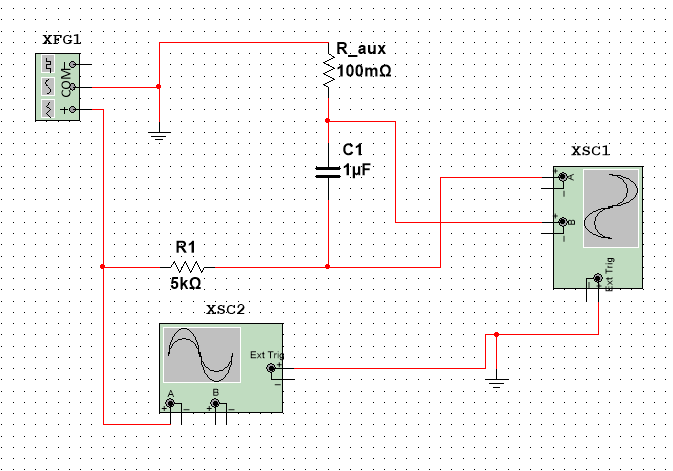
\includegraphics[width=0.6\textwidth]{scheme.png}
    \caption{Схема моделирования.}
    \label{fig:scheme}
\end{figure}

Генератор функций задает прямоугольный сигнал с $f = 10 \ Hz, \ V_{amp} = 10 \ V$. \\
\begin{figure}[H]
    \centering
    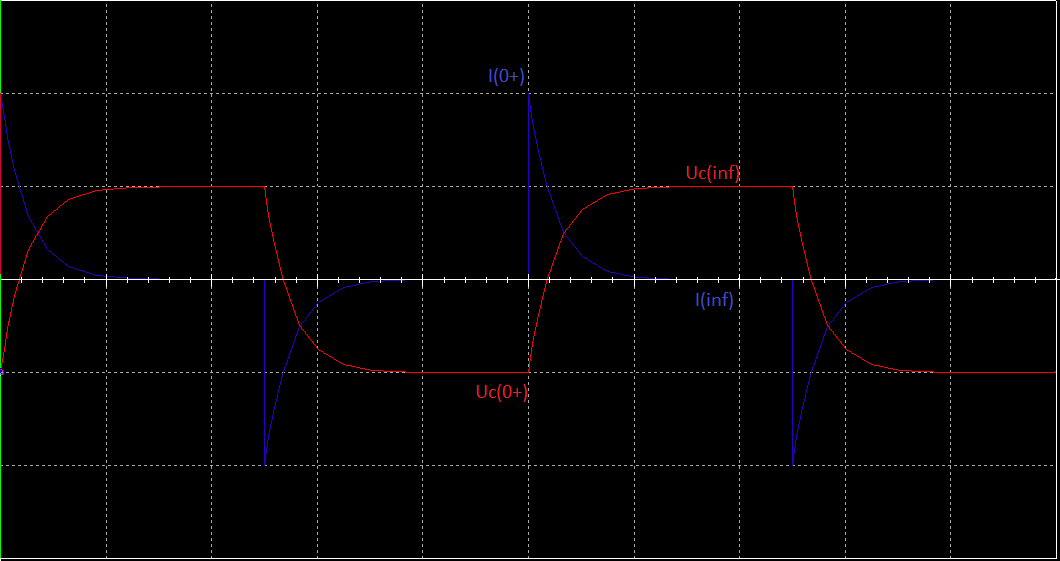
\includegraphics[width=\textwidth]{tran_1.png}
    \caption{Осциллограмма переходного процесса.}
    \label{fig:tran_1}
\end{figure}
\begin{figure}[H]
    \centering
    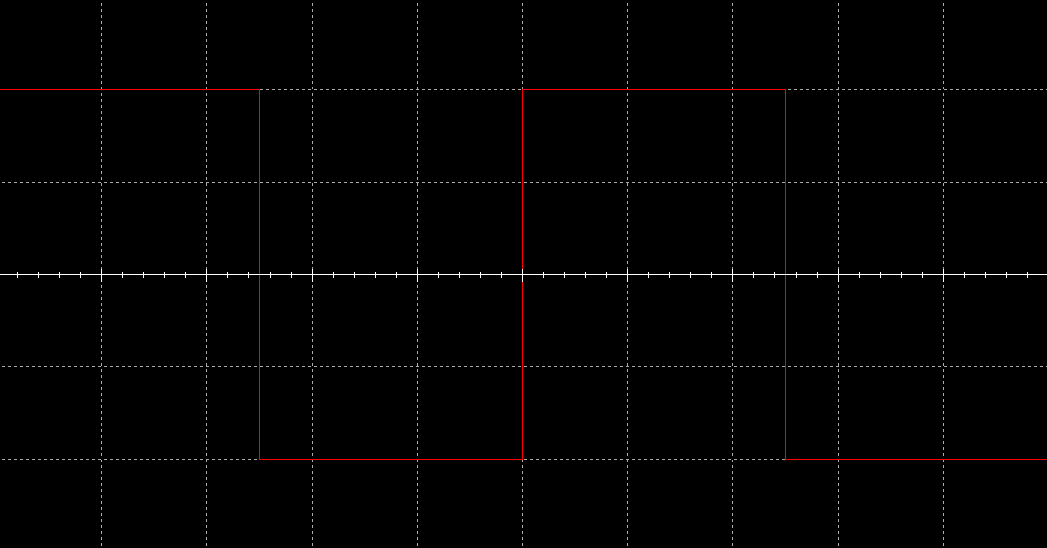
\includegraphics[width=\textwidth]{signal.png}
    \caption{Осциллограмма входного прямоугольного сигнала.}
    \label{fig:signal}
\end{figure}

Произведем аналитический расчет тока $I$ в цепи и напряжения $V_c$ на конденсаторе в моменты коммутации $(t=0+, \ t=0-)$ и установившимся $(t=\infty)$ по следующим формулам:
\[
    V_c(0+) =V_c(0-) = E(0-) = -10 \ V,
\]
\[
    I(0+) = \frac{E+V_c}{R} = 0.4 \ mA.
\]
\[
    V_c(\infty) = E(0+) = 10 \ V,
\]
\[
    I(\infty) = I(0-) = 0 \ A.
\]
Теперь соберем экспериментальные данные с этой схемы:
\[
    I(0+) = 0.3984 \ mA, \ I(\infty) = 3\cdot10^{-12} \ A, \ V_c(0+) = -9.994 \ V, \ V_c(\infty) = 9.989 \ V.
\]
Рассчитаем также постоянную времени:
\[
    \tau = RC = 0.0005 \ sec.
\]

Теперь видоизменим схему, заменив конденсатор катушкой с индуктивностью $L = 1 \ H$ и изменив сопротивление резистора $R_1 = 200 \ Ohm.$
\begin{figure}[H]
    \centering
    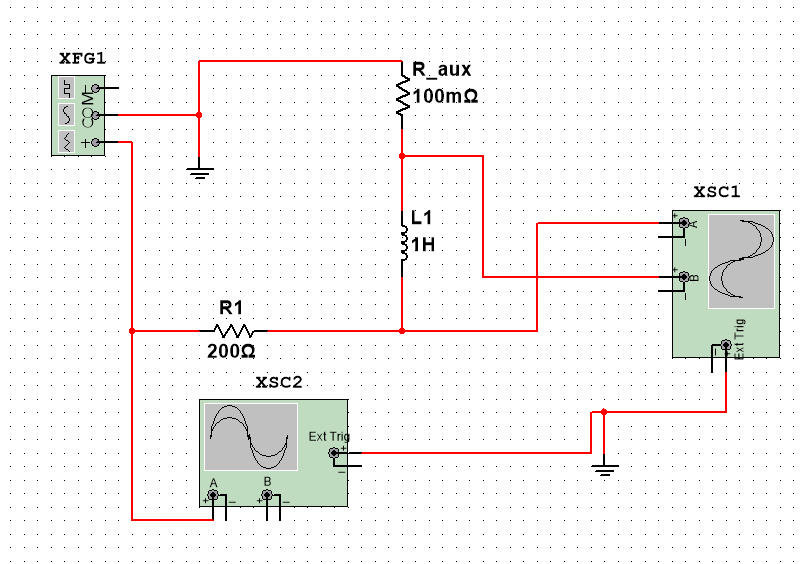
\includegraphics[width=0.6\textwidth]{scheme_2.png}
    \caption{Схема с катушкой индуктивности.}
    \label{fig:scheme_2}
\end{figure}

\begin{figure}[H]
    \centering
    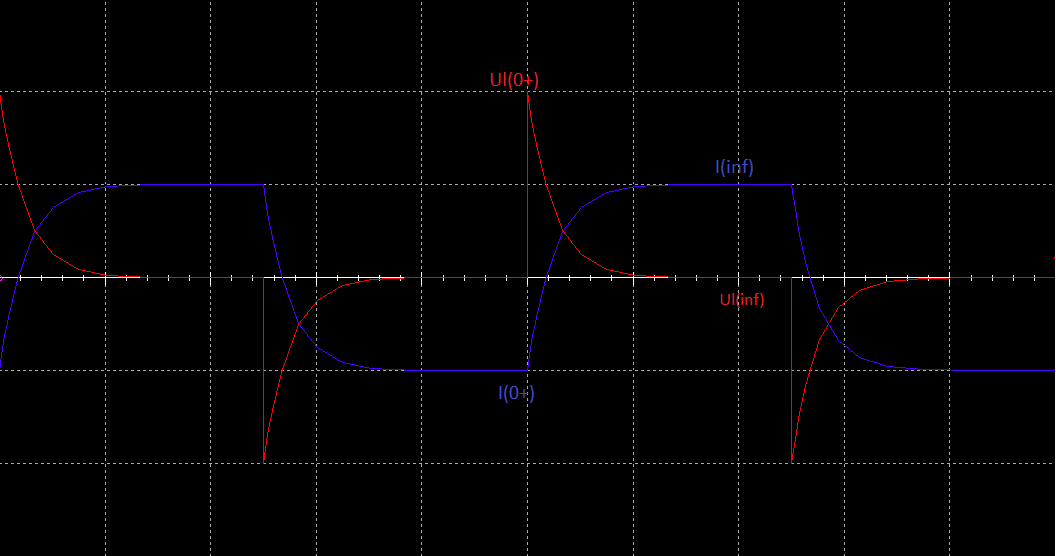
\includegraphics[width=\textwidth]{tran_2.png}
    \caption{Осциллограмма переходного процесса схемы с катушкой.}
    \label{fig:tran_2}
\end{figure}

Произведем аналогичный расчет по следующим формулам:
\[
    V_l(0+) = E(0+) - I(0-) \cdot R = 20 \ V,
\]
\[
    I(0+) = I(0-) = \frac{E(0-)}{R} = -5 \ mA.
\]
\[
    V_l(\infty) = I(inf) \cdot R_k = 5 \ mV,
\]
\[
    I(\infty) = \frac{E(0+)}{R} = 5 \ mA.
\]
Теперь соберем экспериментальные данные с этой схемы:
\[
    I(0+) = -4.995 \ mA, \ I(\infty) = 4.973 \ mA, \ V_l(0+) = 19.98 \ V, \ V_l(\infty) = 5 \ mV.
\]
Рассчитаем также постоянную времени:
\[
    \tau = \frac{L}{R} = 0.005 \ sec.
\]

\subsubsection*{Выводы}
В данной работе были исследованы переходные процессы электрических цепей двух типов: $RL$ и $RC$. \\
Переходные процессы возникают из-за наличия реактивных элементов (соответственно в нашем случае это наличие катушки индуктивности и конденсатора). \\
\ \\
В первой части работы исследовалась цепь с конденсатором. По построенным графикам переходных процессов были выявлены следующие закономерности: ток изменялся по закону убывающей экспоненты (установившееся значение $0 \ A$. А напряжение изменялось от $-10$ до $10 \ V$.
\ \\
Во второй части работы была исследована цепь с катушкой индуктивности. По построенным графикам переходных процессов, мы видим, что ток изменяется от малого значения $-5 \ mA$, до установившегося значения $5\ mA$. А напряжение изменяется по закону отрицательной экспоненты от достаточно большого $20 \ V$ до почти нулевого $5 \ mV$ значения. \\
\ \\
После аналитических вычислений, значения были подкреплены экспериментальными измерениямми, которые совпадали с точностью до неучтенных явлений с вычисленными. \\
Также была вычислена постоянная времени для двух исследоваемых типов цепей, которая является характеристикой зависящей только от физических параметров цепи $R, \ L, \ C$.

\end{document}